The Hazard Modeller's Toolkit (or ''hmtk'') is a Python 2.7 library of functions written by scientists at the GEM Model Facility, which is intended to provide 
scientists and engineers with the tools to help create the seismogenic 
input models that go into the OpenQuake hazard engine. The process of 
developing building the hazard model is a complex and often challenging 
one, and whilst many aspect of the practice are relatively common, the 
choice of certain methods or tools for undertaking each step can be a 
matter of judgement. The intention of this software is to provide 
scientists and engineers with the means to apply many of the most 
commonly used algorithms for preparing seismogenic source models 
using seismicity and geological data. It is still in an early 
stage of development and the current versions contain only a preliminary
set of tools for undertaking the necessary workflows. In forthcoming 
versions will hope to make available more tools for the current processes
indicated here, and to integrate new functionalities for i) merging and
homogenisation of earthquake catalogues, ii) calculation of activity 
rates from geological and geodetic data, iii) testing and interpretation
of Ground Motion Prediction Equations, and iv) integration of 
seismological and geological data and treatment of uncertainty 
in the construction of seismogenic source zones.

\section{The Development Process}

The Hazard Modeller's Toolkit is an activity that has been under development in GEM and has followed different stages. The present decision to make the modelling tools available as a library reflects the general trend in the OpenQuake development process toward having a modular software framework. This means that the modelling - hazard - risk process is separated into libraries (e.g. oq-hazardlib, oq-risklib) that can be utilised as standalone tools, in addition to being integrated within the OpenQuake engine and platform. This is designed to allow for flexibility in the process, to allow the user to begin to utilise (possibly in other contexts) functions and classes that are intended to address particular stages of the calculation. Such an approach ensure that each sub-component of the toolkit is fully tested, with a minimal degree of duplication in the testing process. In the HMTK this is taken a step further as we are aiming to provide the hazard modeller as much control over the modelling process as possible, whilst retaining as complete a level of code testing as is practical to implement given the development resources available. 

The change in the HMTK development process that leads towards the current version is designed to address particular objectives:

\begin{description}
\item[Portability] Reduction in the number of python dependencies to allow for a greater degree of cross-platform deployment than is currently feasible with the main OpenQuake engine

\item[Adaptability] Cleaner separation of methods into self-contained components that can be implemented and tested within requiring adaption of the remainder of the code.

\item[Abstraction] This concept is often a critical component object-oriented development. It describes the specification of a core behaviour of a method, which implementations (by means of the subclass) must follow. For example, a declustering algorithm must follow the common behaviour path, in this instance i) reading and earthquake catalogue and some configurable parameters, ii) identifying the clusters of events, iii) identifying the mainshocks from within each cluster,iv) returning this information to the user. The details of the implementation are then dependent on the algorithm, providing that the core flow is met. This is designed to allow the algorithms to be \emph{interchangeable} in the sense that different methods for  particular task could be selected with no (or at least minimal) modification to the rest of the code.

\item[Usability] The creation of a library which could itself be embedded within larger applications (e.g. as part of a graphical user interface).
 
\end{description}



\section{Getting Started and Running the Software}

The Modeller's Toolkit and associated software are designed for execution 
from the command line. As with OpenQuake, the preferred environment is 
Ubuntu Linux (11.04 or later). A careful effort has been made to keep 
the number of additional dependencies to a minimum. No packaged version of the software has been released at the time of writing, so the user must install the dependencies manually. More information regarding the current dependencies of the toolkit can be found at \hfill \\
\href{http://github.com/GEMScienceTools/hmtk}{http://github.com/GEMScienceTools/hmtk}. 

The current dependencies are:
\begin{itemize}
\item Numpy and Scipy (included in the standard OpenQuake installation)
\item Shapely (included in the standard OpenQuake installation)
\item Openquake nrmllib (included in the standard OpenQuake installation) 
    \hfill \\ (\href{http:/github.com/gem/oq-nrmllib}{http:/github.com/gem/oq-nrmllib}) 
\item Openquake hazardlib (included in the standard OpenQuake installation) 
    \hfill \\ (\href{http:/github.com/gem/oq-hazardlib}{http:/github.com/gem/oq-hazardlib})
\item Matplotlib (\href{http://matplotlib.org/}{http://matplotlib.org/})
\item PyYaml
\item Python Decorator
\end{itemize}

If the OpenQuake Hazard Library (oq-hazardlib) and the OpenQuake Nrml library are already installed on your system (as would be the case if a full installation of the OpenQuake-engine has already been successfully installed) then both dependencies are already available. If this is not the case, however, you will need to install the packages manually. For Linux and OSX users, the recommended approach is to run:

\begin{Verbatim}[frame=single, commandchars=\\\{\}, fontsize=\scriptsize]

~\$ sudo pip install -e https://github.com/gem/oq-hazardlib.git
~\$ sudo pip install -e https://github.com/gem/oq-nrmllib.git

\end{Verbatim}

As of April 2013, the packages have not been tested in a Windows environment, so the recommended approach for windows users would be to use Ubuntu Linux 12.04 within a Virtual Machine.

The Matplotlib, Pyyaml and Decorator dependencies are installed in the library for the demos, but can be installed easy from the command line by:

\begin{Verbatim}[frame=single, commandchars=\\\{\}, fontsize=\scriptsize]

~\$ sudo pip install matplotlib
~\$ sudo pip install pyyaml
~\$ sudo pip install decorator

\end{Verbatim}

To enable usage of the hmtk within any location in the operating system, OSX and Linux users should add the folder location manually to the command line profile file. This can be done as follows:

\begin{enumerate}
\item Using a command line text editor (e.g. VIM), open the \verb=~/.profile= folder as follows:

\begin{Verbatim}[frame=single, commandchars=\\\{\}, fontsize=\scriptsize]
~\$ vim ~/.profile
\end{Verbatim}

\item At the bottom of the profile file (if one does not exist it will be created) add the line:

\begin{Verbatim}[frame=single, commandchars=\\\{\}, fontsize=\scriptsize]
export PYTHONPATH=/path/to/hmtk/folder/:\$PYTHONPATH
\end{Verbatim}

Where \verb=/path/to/hmtk/folder/ is the system path to the location of the hmtk folder (use the command \verb=pwd= from within the hmtk folder to view the full system path).

\item Re-source the bash shell via the command

\begin{Verbatim}[frame=single, commandchars=\\\{\}, fontsize=\scriptsize]
~\$ source ~/.profile
\end{Verbatim}
 
\end{enumerate}

\subsubsection{Windows Installation}

Although this installation has been primarily tested in a Linux/Unix environment it may be possible to install natively in Windows using the following process. This assumes that no other version of Python is installed in your windows environment.

The easiest way to install the OpenQuake hazardlib and nrmllib is by virtue of the PythonXY program \href{http://code.google.com/p/pythonxy/}{http://code.google.com/p/pythonxy/}. This is a free and open python user interface, which will bring in almost all of the dependencies the openquake libraries need. The an installer for the latest version of PythonXY can be downloaded from here: \href{http://code.google.com/p/pythonxy/wiki/Downloads?tm=2}{http://code.google.com/p/pythonxy/wiki/Downloads?tm=2}.

Click on the executable and follow the instructions (the installation may take up to half an hour or more, depending on the system). It is strongly recommended that the use opt for the ``\textbf{FULL}'' installation, which should bring in almost all of the dependencies needed for installing the OpenQuake hazard library. 

For the oq-nrmllib it is necessary to install the Lxml library (\href{http://lxml.de}{http://lxml.de}). This is not officially supported for Windows, so it is recommended (by Python developers themselves!) to install the unofficial Lxml binding from here: \footnote{\href{http://www.lfd.uci.edu/~gohlke/pythonlibs/}{http://www.lfd.uci.edu/~gohlke/pythonlibs/}}. Download and then run the 32-bit package named ``lxml-\#.\#.\#.win32-py2.7.exe''.

Next you will need to install the op-hazardlib and oq-nrmllib. From the web repositories listed previously click the button ``Download Zip'', then extract contents to the folders \verb=C:/oq-hazardlib= and \verb=C:/oq-nrmllib= respectively.

Now open up an enhanced IPython console. Go to Start $->$ Python(xy) $->$ Enhanced Consoles $->$ Ipython (sh). This will open up an Ipython console terminal. To install the oq-hazardlib, at the console prompt type:

\begin{Verbatim}[frame=single, commandchars=\\\{\}, fontsize=\scriptsize]
~\$: cd C:/oq-hazardlib/
~\$: python setup.py install build --compiler=mingw32
\end{Verbatim}

This will install the oq-hazardlib with the full C-extensions, which speed up some of the geometry calculations. Then do the same with the oq-nrmllib.

\begin{Verbatim}[frame=single, commandchars=\\\{\}, fontsize=\scriptsize]
~\$: cd C:/oq-hazardlib/
~\$: python setup.py install
\end{Verbatim}

Then close the console by typing \verb=exit=. 

Finally, download the zipped folder of the hmtk from the github repository and unzip to a folder of your choosing. To allow for usage of the hmtk throughout your operating system, do the following: 

\begin{enumerate}
\item From the desktop, right-click \textbf{My Computer} and open \textbf{Properties}
\item In the ``System Properties'' window click on the \textbf{Advanced} tab.
\item From the ``Advanced'' section open the \textbf{Environment Variables}.
\item In the ``Environment Variables'' you sill see a list of ``System Variables'', select ``Path'' and ``Edit''.
\item Add the path to the hmtk directory to the list of folders then save.
\end{enumerate}

After this process it may be necessary to restart PythonXY.



%\textbf{For the purposes of the current exercises all of the Modeller's Toolkit dependencies have been installed in both the OpenQuake .ova files and on the OATS server - so no installation is necessary! For instructions on how to install OpenQuake and the Modeller's Toolkit, please refer to the appendix of this document}

\subsection{Current Features}

The Hazard Modeller's Toolkit is currently divided into three sections, which can be used interactively: 

\begin{enumerate}
\item \textbf{Earthquake Catalogue and Seismicity Analysis}
    These functions are intended to address the needs of defining seismic activity rate from an earthquake catalogue. They algorithms for identification of Non-Poissonian events (declustering), analysis of catalogue completeness, calculation of activity rate and b-value and, finally, estimation of maximum magnitude using statistical analyses of the earthquake catalogue. Also included in these tools is an initial implementation of a smoothed seismicity algorithm using the \cite{frankel1995} approach.
     
\item \textbf{Active Faults Source Models from Geological Data}

    These functions are intended to address the Modeller needs for defining earthquake activity rates on fault sources from the geological slip rate, including support for some epistemic uncertainty analysis on critical parameters in the process.

\item \textbf{Seismic Source Models from Geodetic Data}

    These functions are intended to address the use of geodetic data to derive seismic activity rates from a strain rate model for a region, implementing the Seismic Hazard Inferred from Tectonics (SHIFT) methodology developed by \cite{BirdLiu2007} and applied on a global scale by\cite{Bird_etal2010}.
\end{enumerate}

A summary of the algorithms available in the present version (V0.1) is given in Table 
\begin{table}
\begin{tabular}{|c|c|} \hline
Feature & Algorithm\\ \hline
\textbf{Seismicity} & \\ \hline
Declustering & \cite{GardnerKnopoff1974}  \\
    & AFTERAN (\cite{Musson1999}) \\ \hline
Completeness & \cite{Stepp1971}\\ \hline
Recurrence & Maximum Likelihood \cite{Aki1965}\\
 & Time-dependent MLE\\
 & \cite{Weichert1980}\\ \hline
 Smoothed Seismicity & \cite{frankel1995} \\ \hline
 \textbf{Geology} & \\ \hline
 Recurrence & \cite{AndersonLuco1983} ``Arbitrary''\\
  & \cite{AndersonLuco1983} ``Area $M_{MAX}$''\\
  & Characteristic (Truncated Gaussian) \\
  & \cite{YoungsCoppersmith1985} Exponential\\
  & \cite{YoungsCoppersmith1985} Characteristic\\ \hline
 \textbf{Geodetic Strain} & \\ \hline
 Recurrence & Seismic Hazard Inferred from Tectonics (SHIFT) \\
           &  \cite{BirdLiu2007, Bird_etal2010} \\ \hline
\end{tabular}
\end{table}

\subsection{About this Tutorial}

As previously indicated, the Modeller's Toolkit itself is a Python library. This means that its functions can be utilised in many different python applications. It is not, at present, a stand-alone software, and requires some investment of time from the user to understand the functionalities and learn how to link the various tools together into a workflow that will be suitable for the modelling problem at hand.

This manual is designed to explain the various functions in the toolkit and to provide some illustrative examples showing how to implement them for particular contexts and applications. The tutorial itself does not specifically require a working knowledge of Python. However, an understanding of the basic python data types, and ideally some familiarity with the use of Python objects, is highly desirable. A good overview of the features of the python programming language can be found in the standard python documentation (\href{http://docs.python.org/2/tutorial/}{http://docs.python.org/2/tutorial/}). Where necessary particular Python programming concepts will be explained in further detail.

The code snippets (indicated by verbatim text) can be executed from within an ''Interactive Python'' environment, or may form the basis for usage of the hmtk in other python scripts that the user may wish to run construct themselves. If not already installed on your system, ipython can be installed from the python package repository by entering: 

\begin{Verbatim}[frame=single, commandchars=\\\{\}, fontsize=\scriptsize]

~\$ sudo pip install ipython

\end{Verbatim}

%For the current exercise of preparing seismic hazard inputs for sources in Nepal, a "wrapper" script has been prepared that links together a common workflow: 

\begin{enumerate}

\item Starting with a single magnitude-homogenised earthquake catalogue apply a declustering algorithm to identify and remove non-Poissonian events

\item For the declustered catalogue, use a statistical methodology to determine the time variation in completeness. Currently only the methodology of \cite{Stepp1971} is implemented.

\item With the completeness periods of the catalogue known calculate a \cite{GutenbergRichter1944} recurrence model (a- and b-value with uncertainties) for either the catalogue as a whole, or for earthquakes selected within certain area zones.

\item Implementation of a statistical estimator of maximum magnitude from the earthquake catalogue  

\end{enumerate}

An "interactive" session can then be opened by typing \verb=ipython= at the command prompt. If matplotlib is installed and you want to make use of one or two of the plotting functionalities then you should open ipython with \verb=ipython --pylab=. To exit an ipython session at any time simply type \verb=exit=.

The Modeller's Toolkit itself requires no specific installation. In a Unix/Linux environment you can simply download the code as a zipped package from the website shown previously, then unzip and move into the code directory.
Alternatively you can download the code directly into  any current repository with the command

\begin{Verbatim}[frame=single, commandchars=\\\{\}, fontsize=\scriptsize]

~\$ git clone https://github.com/GEMScienceTools/hmtk.git

\end{Verbatim}


%The execution of the Modeller's Toolkit is done from within the main directory in which the code is contained. The selection of the algorithm and the general configuration of the software is done via a configuration file (in this example \verb=Nepal_hmtk_demo_config.yml=. This is a YAML (Yet Another Markup Language) file, which can be opened and edited with any common text editor (e.g. vi, emacs, gedit).
%
%To run the Nepal "wrapper" code for the Modeller's Toolkit simply move into the directory in which the \verb=main.py= file is found. Once the configuration file is correctly set up, execute via the following command:
%\begin{Verbatim}[frame=single, commandchars=\\\{\}, fontsize=\scriptsize]
%~\$ python hmtk_Nepal_Demo.py --input=Nepal_hmtk_demo_config.yml
%\end{Verbatim}

%The \verb=-d= indicates that the program can be run in ''debug'' mode. This will create a log (written automatically to the file \verb=debug.log=) of the processes that are executed inside the toolkit in addition to certain parameters that may be calculated at intermediate steps of the process, but are not written to the output. The \verb=-d= can be omitted if preferred, in which case the program will return only a minimal indication of the progress to the command prompt.

%\subsection{Nepal Demonstration: The Configuration File}
%
%The following demonstration is designed to illustrate how the toolkit could be used to help build a hazard model using current data (and seismogenic sources) for Nepal and the surrounding regions. The data and the study area are shown in Figure \ref{fig:KathGSHAPLabel}
%
%\begin{figure}[htbp]
%	\centering
%		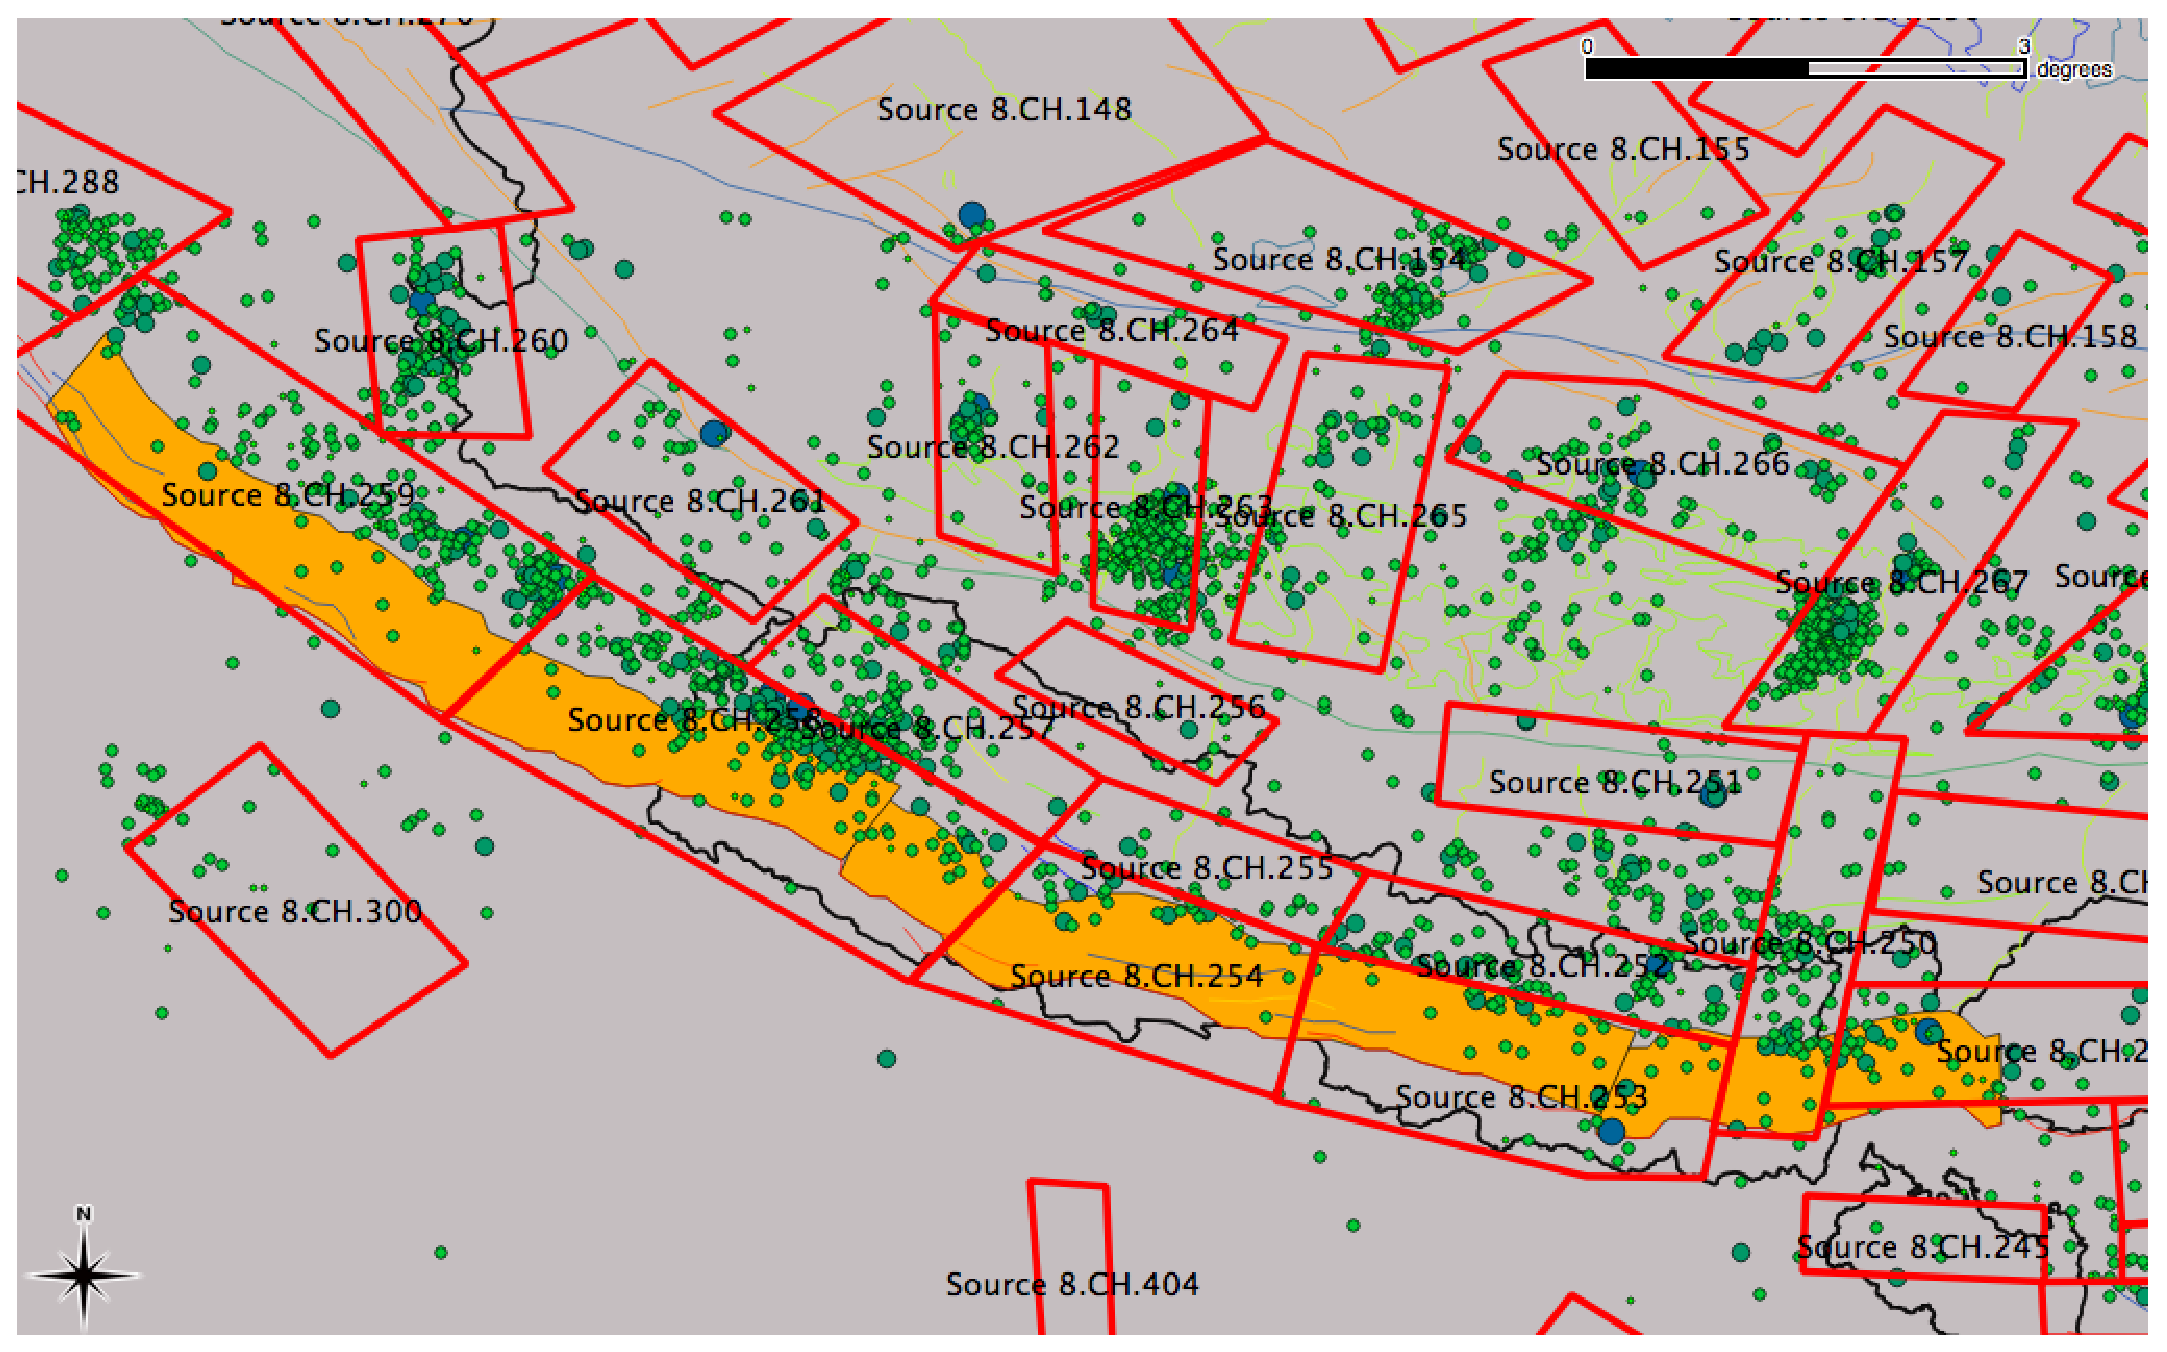
\includegraphics[width=15cm, keepaspectratio=true]{./figures/Kathmandu_plus_GSHAP_sources_labelled.eps}
%	\caption{Seismotectonic Information for Nepal and the Surroundings. Earthquakes catalogue taken from the International Seismological Centre, Area Sources (red) from GSHAP and active fault sources (including surface projections for the Main Boundary Thrust (orange)) from \cite{TaylorYin2009}}
%	\label{fig:KathGSHAPLabel}
%\end{figure}






